\section{EJERCICIO 2.2: HDL decodificador BCD}\sangria{} El objetivo de este ejercicio es describir en Verilog HDL el comportamiento completo del decodificador BCD a 7 segmentos.\subsection{Materiales utilizados}\begin{itemize}[nosep]\item Kit CPLD. \item Software Xilinx.\end{itemize}\subsection{Procedimiento}\begin{enumerate}[nosep]\item Se describió en HDL Verilog. \item Sintetizó para obtener el RTL para el CPLD XC9582XL. \item UCF: \begin{itemize}[nosep]\item Identificar los pines del display de 7 segmentos. \item Identificar el transistor que activa el display. \item Identificar la llave a usar. \end{itemize}\item Se implementó el diseño y la simulación. \item Conectado de CPLD y la fuente de alimentación. \item Borrado del viejo CPLD desde Manager Configuration Project y cargado del binario JED. \end{enumerate}
\begin{center}\begin{figure}[h!]
\centering
\begin{subfigure}[b]{0.45\linewidth}
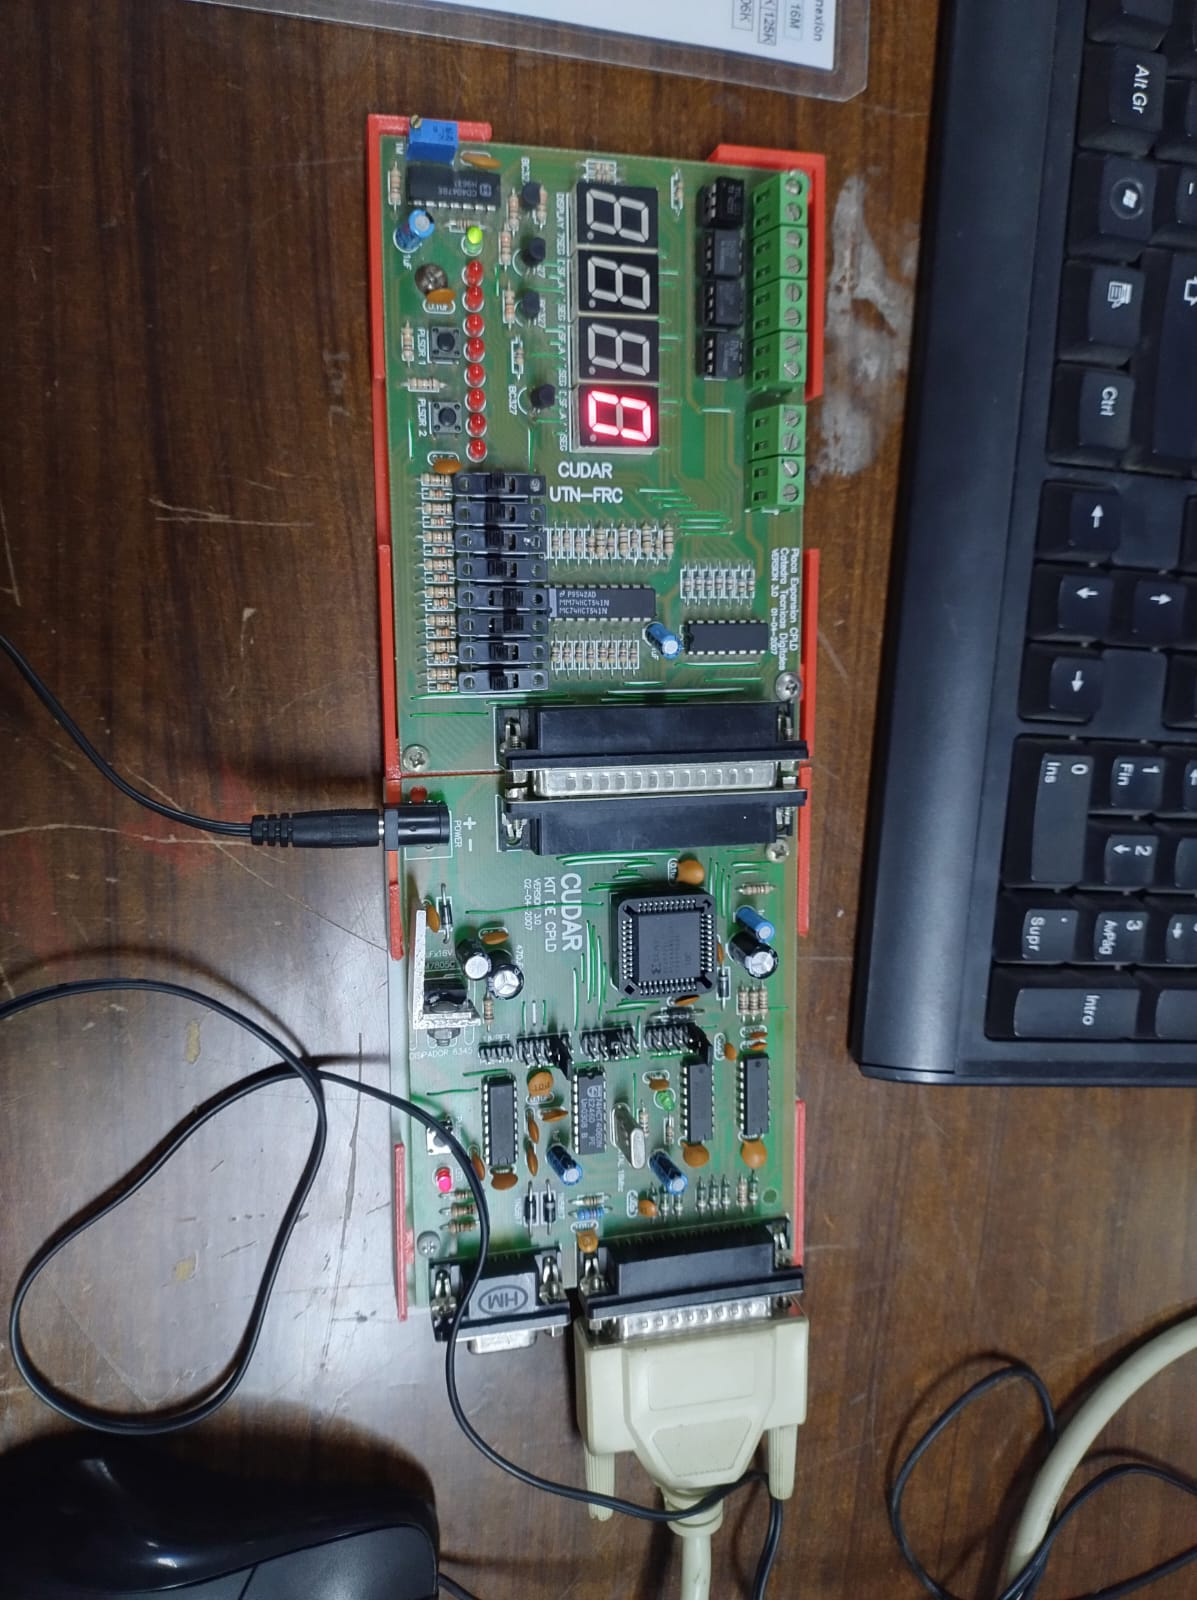
\includegraphics[width=\linewidth]{./imagenes/0CPLD.jpg}
\caption{1 - CPLD}
\label{fig:westminster_lateral}
\end{subfigure}
\begin{subfigure}[b]{0.45\linewidth}
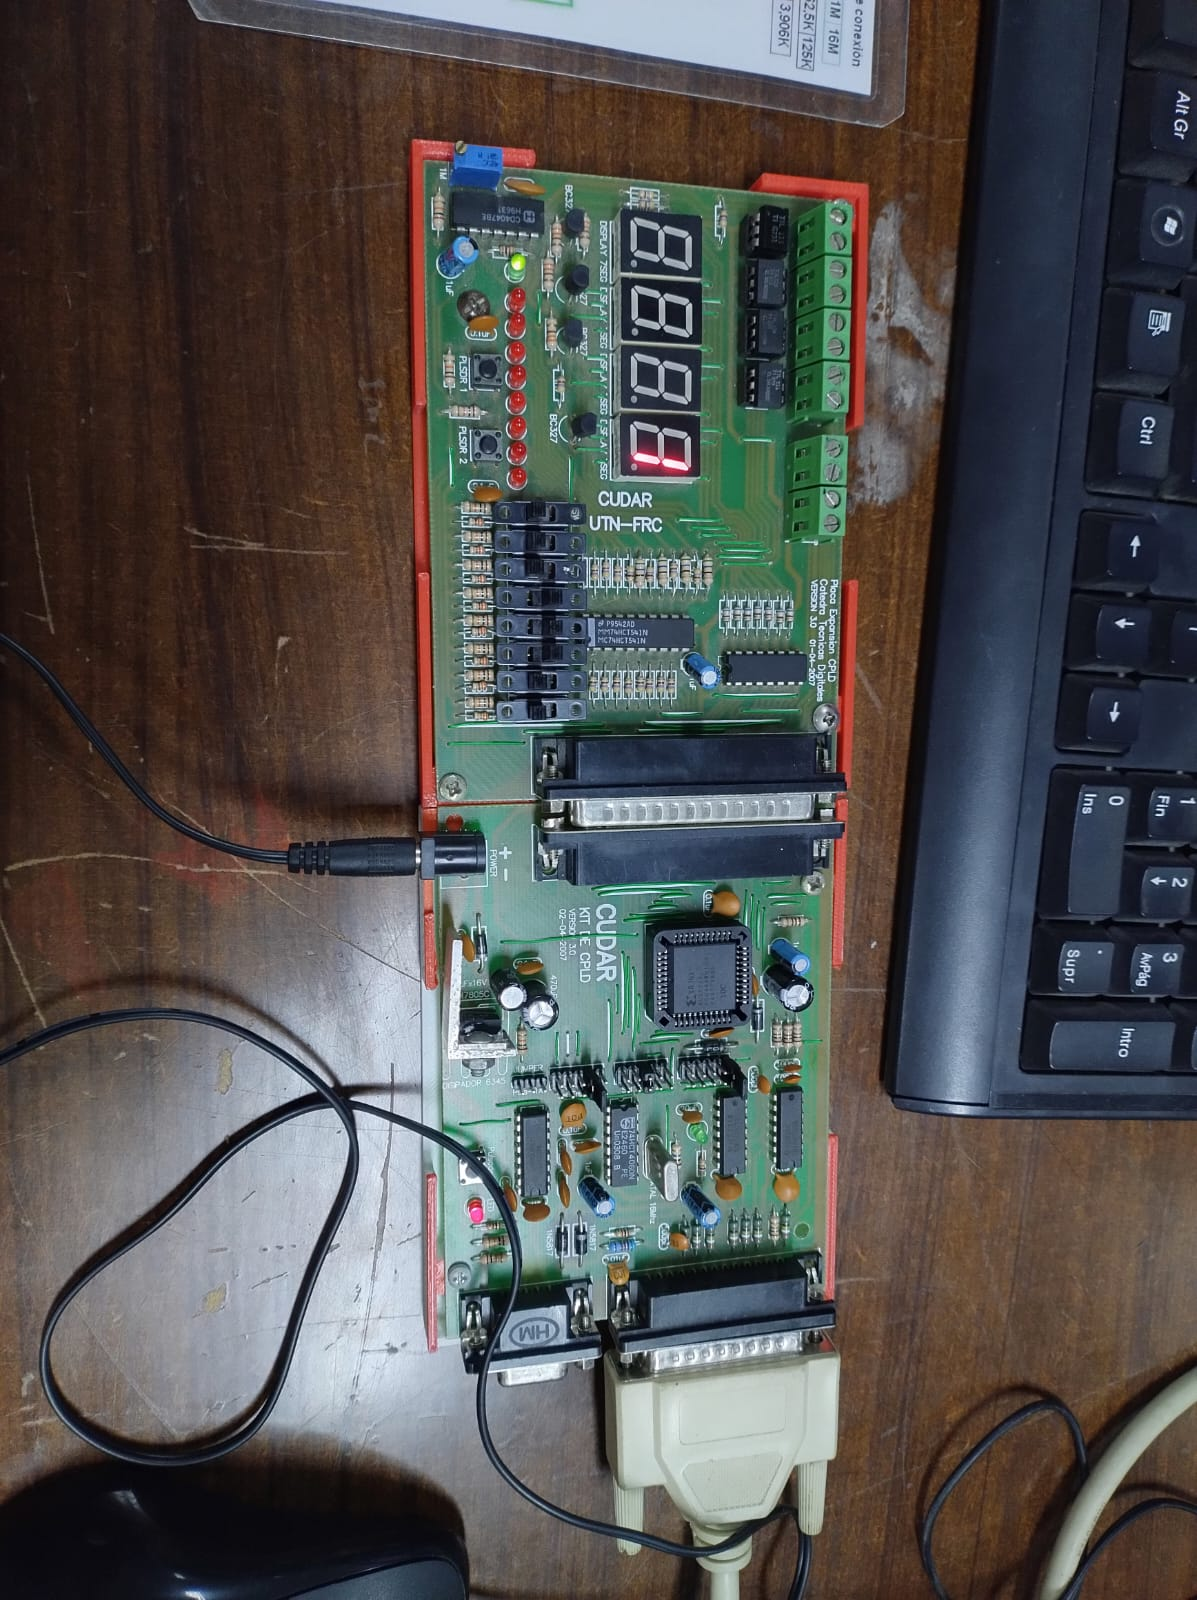
\includegraphics[width=\linewidth]{./imagenes/1CPLD.jpg}
\caption{1 - CPLD}
\label{fig:westminster_aerea}
\end{subfigure}
\caption{Algunos digitos del CPLD}
\label{fig:westminster}
\end{figure}\end{center}

\subsection{Código HDL Verilog}
\begin{lstlisting}
module bcdTo7Seq(
    input [3:0] BCD,
    input LT, BL,
    output mosfet,
    output reg [6:0] display
);

assign mosfet = 0;

always @(*) begin
    if (!LT)
        display = 7'b1111111;
    else if (!BL)
        display = 7'b0000000;
    else begin
        case (BCD)
            4'd0: display = 7'b1111110;
            4'd1: display = 7'b0110000;
            4'd2: display = 7'b1101101;
            4'd3: display = 7'b1111001;
            4'd4: display = 7'b0110011;
            4'd5: display = 7'b1011011;
            4'd6: display = 7'b1011111;
            4'd7: display = 7'b1110000;
            4'd8: display = 7'b1111111;
            4'd9: display = 7'b1110011;
            default: display = 7'b0000000;
        endcase
    end
end

endmodule
\end{lstlisting}
